\section{Вычислимость}

\subsection{Композиция вычислимых функций вычислима}
Пусть машина $M_f$ вычисляет функцию f, а машина $M_g$ — функцию g. Тогда функцию f(g(x)) можно вычислить машиной $M_g$, которая вместо своего конечного
состояния переходит в начальное состояние машины $M_f$ (при этом для самой машины
$M_f$ нужны новые состояния, не пересекающиеся с состояниями $M_f$).

\subsection{Существование невычислимых функций, неразрешимых и неперечислимых множеств}
\textbf{Невычислимая}\\
Функции, о которых идет речь, представляют собой функции, заданные и принимающие значения в множестве слов в алфавите А. Ясно, что множество слов в алфавите А счетно. Следовательно, рассматривается множество всех функций, заданных на счетном множестве и принимающих значения в счетном же множестве. Как известно, это множество имеет мощность континуума. С другой стороны, поскольку множество всевозможных машин Тьюринга счетно, то множество функций, вычислимых по Тьюрингу, также счетно. Континуальная мощность строго больше счетной. Следовательно, существуют функции, не вычислимые по Тьюрингу.
\\
\textbf{Неразрешимое и неперечислимое множество}\\
Алгоритмов (и поэтому разрешимых/перечислимых подмножеств натурального ряда) счётное число, а всех подмножеств натурального ряда несчётное число. Значит, из соображения мощности найдутся неразрешимые и неперечислимые множества

\subsection{Перечислимость любого разрешимого множества}
По определению разрешимого множества, существует такая машина, что если $x \in A$, то существует вычисление, начинающееся в $q_1x$ и заканчивающееся в $q_a$. Это значит, что для этой машины все $x \in A$ встречаются в потоке вывода. Значит, множество A перечислимо

\subsection{Разрешимость любого конечного множества.}
Алгоритм разрешения любого конечного множества S содержит таблицу элементов множества S, вход сравнивается по очереди со всеми элементами таблицы. В случае совпадения выдаем 1, иначе 0

\subsection{Замкнутость классов разрешимых и перечислимых множеств относительно пересечения и объединения, класса разрешимых относительно дополнения}
\textbf{Пересечение и объединение перечислимых множеств - перечислимое множество}
\\
Если X и Y перечисляются алгоритмами A и B, то их объединение перечисляется алгоритмом, который параллельно выполняет по шагам A и B и печатает всё, что печатают A и B. С пересечением немного сложнее — результаты работы A и B надо накапливать и сверять друг с другом; что появится общего — печатать.

\textbf{Пересечение, объединение, дополнение разрешимых множеств - разрешимое множество}\\
Пересечение, объединение, дополнение - это просто композиция соответствующей характеристической функции и булевой функции.
\begin{itemize}
    \item Для дополнения достаточно рассмотреть тот же алгоритм, что я для разрешения множества A. Вместо единицы печатать 0, вместо 0 - единицу.
    \item $\chi_{A \cup B}(x) = \chi_A \vee \chi_B$ - вычислима
    \item $\chi_{A \cap B}(x) = \chi_A \wedge \chi_B$ - вычислима
\end{itemize}

\subsection{Существование вычислимой в обе стороны биекции между $\mathbb{N}^2$ и $\mathbb{N}$}
$(x,y) \mapsto (2x + 1)2^y$
\\
Это биекция - очевидно, так как любое число представимо таким образом,причем разным числам соответствуют разные представления, и для любого числа вида $(2x + 1)2^y$ найдется число из N. 
\\
Опишем алгоритм вычисления
\begin{itemize}
    \item [=>] Очевидно, такая функция вычислима, как функция от двух аргументов
    \item[<=] Делим число на 2, пока оно четно. Получаем отсюда у. Потом вычитаем один, делим на 2, получаем х. 
\end{itemize}
Таким образом, построенная биекция вычислима в обе стороны, а значит, подходит под условие

\subsection{Подмножество разрешимого (перечислимого) множества не обязательно разрешимо (перечислимо), и наоборот}
\textbf{Подмножество разрешимого/перечислимого множества может быть неразрешимо/неперечислимо}
\\
Любое множество, в т.ч. неразрешимое/неперечислимое, является подмножеством $\mathbb{N}$, которое разрешимо/перечислимо
\\
\textbf{Подмножество неразрешимого/неперечислимого множества может быть разрешимо/перечислимо}
Достаточно в любом множестве выбрать конечное подмножество, тогда оно разрешимо/перечислимо

\subsection{Свойства m-сводимости: транзитивность, сводимость дополнений, разрешимость
множества, m-сводимого к разрешимому, перечислимость множества, m-сводимого
к перечислимому}
\begin{center}
    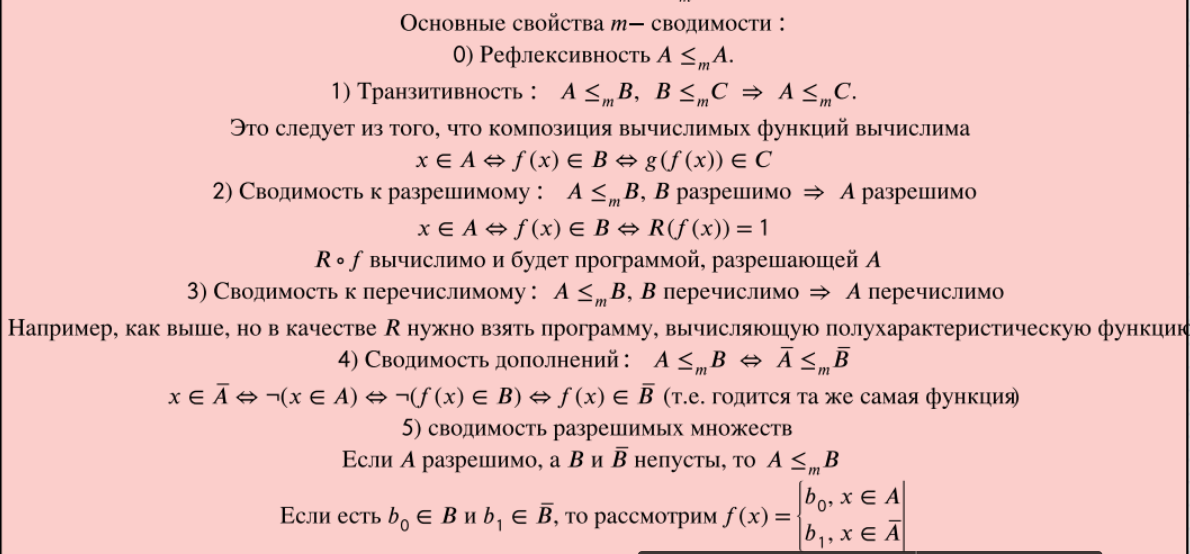
\includegraphics[width = 17cm, height = 6.5cm]{images/3 (определения)_m34.PNG}
\end{center}

\subsection{Вложенность классов в арифметической иерархии}
$\Sigma_k \subset \Sigma_{k+1}, \Sigma_k \subset \Pi_{k+1}, \Pi_k \subset \Sigma_{k+1}, \Pi_k \subset \Pi_{k+1} \\ \blacktriangle$ Добавляем нужный квантор по фиктивной переменной. Например, $\exists y (x,y) \in R \Longleftrightarrow \exists y \forall z (x,y,z)\in R \times \mathbb{N} \Longleftrightarrow \forall t \exists y (x,y,t) \in R\times \mathbb{N}$ (из $\Sigma_1$ в $\Pi_2, \Sigma_2$) $\ \blacksquare$

\subsection{Замкнутость классов арифметической иерархии относительно объединения и пересечения}
Пусть $A,B \in \Sigma_k$
\begin{center}
    $x \in A \Leftrightarrow \exists y_1\ \forall y_2 ... \exists y_k (x,y_1,...,y_k) \in R$ \\
    $x \in B \Leftrightarrow \exists z_1\ \forall z_2 ... \exists z_k (x,z_1,...,z_k) \in Q$
    \\
    $x \in A \cap B \ \Longleftrightarrow (\exists y_1\ \forall y_2 ... \exists y_k (x,y_1,...,y_k) \in R) \ \vee \ (\exists z_1\ \forall z_2 ... \exists z_k (x,z_1,...,z_k) \in Q)  \Longleftrightarrow \ \exists(y_1,z_1) \forall (y_2,z_2) ... \exists(y_k,z_k)((x,y_1,...,y_k) \in R \wedge (x,z_1,...,z_k) \in Q)$ 
\end{center}
что является разрешимым свойством следующего кортежа: ($(x,(y_1,z_1),...,(y_k,z_k)$).\\ Значит, $A \cap B \in \Sigma_k$. Для объединения аналогично.

\subsection{Пример $\lambda$-терма, к которому можно применить $\beta$-редукцию только после $\alpha$-конверсии}
$(\lambda xy.x)y \underset{\alpha}{\Longrightarrow}(\lambda xt.x)y \underset{\beta}{\Longrightarrow}\lambda t.y$

\subsection{Пример $\lambda$-терма, не имеющего нормальной формы} $(\lambda x.xx)(\lambda x.xx)$

\subsection{Построение комбинаторов сложения и умножения для нумералов Чёрча (с доказательством корректности)} 
 Add - сложение.\\
 Add $\overline{mn}$= $(\lambda mn fx. mf(nfx))\overline{m}\overline{n} = (\lambda n fx.\overline{m}f(nfx))\overline{n} = (\lambda n fx.(\lambda gy.\underbrace{g(g...(g}_{m}y)...))f(nfx))\overline{n} = (\lambda n fx.(\lambda y.\underbrace{f(f...(f}_{m}y)...))(nfx))\overline{n} = \lambda fx.(\lambda y.\underbrace{f(f...(f}_{m}y)...))(\overline{n}fx) = \\ \lambda fx.(\lambda y.\underbrace{f(f...(f}_{m}y)...))(\lambda gt.\underbrace{g(g...(g}_{n}t)...))fx) =  \lambda fx.(\lambda y.\underbrace{f(f...(f}_{m}y)...))(\underbrace{f(f...(f}_{n}x)...))) = \\ \lambda fx.(\underbrace{f(f...(f}_{m + n}x)...)) = \overline{m} +\overline{n}$ \\
\\
Mult - умножение:\\
    $Mult \ \overline{mn} = (\lambda mn fx. m(nf)x)\overline{mn} =  (\lambda n fx. \overline{m}(nf)x)\overline{n} = (\lambda n fx. (\lambda gy.\underbrace{g(g...(g}_{m}y)...))(nf)x)\overline{n} \\ = \lambda fx. (\lambda gy.\underbrace{g(g...(g}_{m}y)...))(\overline{n}f)x = \lambda fx. (\lambda y.\underbrace{\overline{n}f(\overline{n}f...(\overline{n}f}_{m}y)...))x = \\ \lambda fx. (\lambda y.\underbrace{\overline{n}f(\overline{n}f...\overline{n}f(\lambda g t_1. \underbrace{g(g...(g}_{n}t_1)...))f}_{m}y)...))x \\ = \lambda fx. (\lambda y.\underbrace{\overline{n}f(\overline{n}f...\overline{n}f}_{m-1}(\underbrace{f(f...(f}_{n}y)...)))...))x  = \lambda fx. (\lambda y.\underbrace{\overline{n}f(\overline{n}f...\overline{n}f}_{m-2}(\underbrace{f(f...(f}_{n + n}y)...)))...))x = ... = \\ \lambda fx. (\lambda y.(\underbrace{f(f...(f}_{n*m}y)...)))...))x = \lambda fx.\underbrace{f(f...(f}_{n*m}x)..) = \overline{m}*\overline{n} $
    \subsection{Extra}
Вопрос Шеня: существует ли вычислимая функция, равная в нуле единице? Ответ: ага. $f(x) = x + 1$